\documentclass[10pt]{article}
% =========================================================
%                PAQUETES DE CONFIGURACIÓN
% =========================================================
\usepackage[T1]{fontenc}
\usepackage[utf8]{inputenc}
\usepackage[english,spanish]{babel}
\usepackage[
paperwidth=28cm,
paperheight=15.75cm,
top=0.18cm,
bottom=0.18cm,
left=0.35cm,
right=0.35cm
]{geometry}
\usepackage{xcolor}
\usepackage{setspace}
\usepackage{graphicx}
\usepackage{amsmath,amssymb}
\usepackage{hyperref}
\usepackage[many]{tcolorbox}
\usepackage{tikz}
\usetikzlibrary{shapes.geometric,calc}
\usepackage{ragged2e}
\usepackage{csquotes}
\usepackage{mathpazo}
\usepackage{microtype}
\usepackage{enumitem}
% =========================================================
%            ENTORNO PERSONALIZADO PARA EXTRACCIÓN A JS
% =========================================================
\newenvironment{extraer}[1]{}{}
% =========================================================
%                    CONFIGURACIÓN GENERAL
% =========================================================
\pagestyle{empty}
\setstretch{0.80}
\hypersetup{colorlinks=false}
\setlength{\parindent}{0pt}
\setlength{\parskip}{0pt}
\setlist{nosep,leftmargin=*}
% =========================================================
%                            COLORES
% =========================================================
\definecolor{deepblue}{RGB}{12,20,38}
\definecolor{gold}{RGB}{176,140,52}
\definecolor{golddark}{RGB}{120,90,22}
\definecolor{goldlight}{RGB}{225,205,145}
\definecolor{heartred}{RGB}{158,30,45}
\definecolor{burgundy}{RGB}{85,18,30}
\definecolor{textgray}{RGB}{35,33,30}
\definecolor{cream}{RGB}{253,250,244}
\definecolor{creamdark}{RGB}{244,237,222}
\definecolor{softgold}{RGB}{238,222,180}
\definecolor{framegold}{RGB}{162,128,42}
% =========================================================
%            SÍMBOLOS TIKZ (ULTRALIGEROS Y VECTORES)
% =========================================================
\newsavebox{\boxCruz}
\newsavebox{\boxCruzInvertida}
\newsavebox{\boxCorazonRojo}
\newsavebox{\boxCerebro}
\newsavebox{\boxCuantica}
\sbox{\boxCruz}{%
	\tikz[baseline=-0.35ex,scale=0.50]{
		\fill[golddark] (-0.09,0.42) rectangle (0.09,-0.48);
		\fill[golddark] (-0.28,0.18) rectangle (0.28,0.36);
		\fill[gold!88] (-0.07,0.40) rectangle (0.07,-0.46);
		\fill[gold!22] (-0.26,0.20) rectangle (0.26,0.34);
	}%
}
\sbox{\boxCruzInvertida}{%
	\tikz[baseline=-0.15ex,scale=0.50,rotate=180]{
		\fill[golddark] (-0.09,0.42) rectangle (0.09,-0.48);
		\fill[golddark] (-0.28,0.18) rectangle (0.28,0.36);
		\fill[gold!65] (-0.07,0.40) rectangle (0.07,-0.46);
		\fill[gold!65] (-0.26,0.20) rectangle (0.26,0.34);
	}%
}
\sbox{\boxCorazonRojo}{%
	\tikz[baseline=-0.25ex,scale=0.35]{
		\fill[heartred]
		(0,-0.55)
		.. controls (-0.55,-0.15) and (-0.55,0.45) .. (0,0.25)
		.. controls (0.55,0.45) and (0.55,-0.15) .. (0,-0.55);
		\fill[heartred!65!white,opacity=0.30]
		(-0.12,0.05) circle (0.11);
	}%
}
\sbox{\boxCerebro}{%
	\tikz[baseline=-0.2ex,scale=0.30]{
		\fill[burgundy]
		(0,0.55)
		.. controls (-0.55,0.55) and (-0.7,0.1) .. (-0.55,-0.25)
		.. controls (-0.4,-0.55) and (-0.15,-0.55) .. (0,-0.4)
		.. controls (0.15,-0.55) and (0.4,-0.55) .. (0.55,-0.25)
		.. controls (0.7,0.1) and (0.55,0.55) .. (0,0.55);
		\draw[cream,line width=0.65pt]
		(-0.35,0.15) .. controls (-0.1,0.35) and (0.1,0.0) .. (0.35,0.2);
		\draw[cream,line width=0.5pt]
		(-0.25,-0.15) .. controls (0.0,0.05) and (0.15,-0.25) .. (0.3,-0.05);
	}%
}
\sbox{\boxCuantica}{%
	\tikz[baseline=-0.3ex,scale=0.40]{
		\draw[golddark, line width=0.7pt, rotate=30] (0,0) ellipse (0.6cm and 0.25cm);
		\draw[golddark, line width=0.7pt, rotate=-30] (0,0) ellipse (0.6cm and 0.25cm);
		\draw[golddark, line width=0.7pt] (0,0) circle (0.35cm);
		\fill[gold!90] (0,0) circle (0.15cm);
		\fill[cream] (0,0) circle (0.06cm);
	}%
}
\newcommand{\cruz}{\usebox{\boxCruz}}
\newcommand{\cruzinvertida}{\usebox{\boxCruzInvertida}}
\newcommand{\corazonrojo}{\usebox{\boxCorazonRojo}}
\newcommand{\cuantica}{\usebox{\boxCuantica}}
\newcommand{\cerebro}{\usebox{\boxCerebro}}
% =========================================================
%                    MARCO DE LA PÁGINA
% =========================================================
\newcommand{\marcoPagina}{%
	\begin{tikzpicture}[remember picture,overlay]
		\fill[cream] (current page.south west) rectangle (current page.north east);
		\draw[framegold,line width=1.5pt]
		([xshift=0.22cm,yshift=-0.22cm]current page.north west)
		rectangle
		([xshift=-0.22cm,yshift=0.22cm]current page.south east);
		\draw[goldlight!80!gold,line width=0.5pt]
		([xshift=0.38cm,yshift=-0.38cm]current page.north west)
		rectangle
		([xshift=-0.38cm,yshift=0.38cm]current page.south east);
		\draw[gold!30,line width=0.25pt]
		([xshift=0.48cm,yshift=-0.48cm]current page.north west)
		rectangle
		([xshift=-0.48cm,yshift=0.48cm]current page.south east);
		\foreach \corner/\dx/\dy in {
			north west/0.22cm/-0.22cm,
			north east/-0.22cm/-0.22cm,
			south west/0.22cm/0.22cm,
			south east/-0.22cm/0.22cm
		}{
			\draw[gold!70!black,line width=0.8pt] ([xshift=\dx,yshift=\dy]current page.\corner) circle (3.8pt);
			\draw[goldlight,line width=0.35pt] ([xshift=\dx,yshift=\dy]current page.\corner) circle (5.3pt);
			\fill[golddark] ([xshift=\dx,yshift=\dy]current page.\corner) circle (1.4pt);
		}
	\end{tikzpicture}%
}
% =========================================================
%                    ESTILOS DE CAJAS
% =========================================================
\tcbset{
	sideStyle/.style={
		enhanced, colback=cream!98, colframe=gold!60!black,
		boxrule=0.65pt, arc=3pt, valign=center,
		left=2pt, right=2pt, top=1pt, bottom=1pt,
		borderline={0.2pt}{0.9pt}{gold!30}
	},
	titleBoxStyle/.style={
		enhanced, colback=gold!5!cream, colframe=gold!85!black,
		boxrule=0.85pt, arc=4pt, top=1.2pt, bottom=1.2pt, left=3pt, right=3pt,
		halign=center, borderline={0.3pt}{1.1pt}{gold!40}
	},
	contentStyle/.style={
		enhanced, colback=cream!99, colframe=gold!50!black,
		boxrule=0.65pt, arc=3.5pt, top=1.2pt, bottom=1.2pt, left=2.8pt, right=2.8pt,
		borderline={0.2pt}{0.9pt}{gold!22}
	},
	centralStyle/.style={
		enhanced, colback=cream!98, colframe=gold!60!black,
		boxrule=0.65pt, arc=3.5pt, top=1.2pt, bottom=1.2pt, left=2.8pt, right=2.8pt,
		borderline={0.25pt}{0.9pt}{gold!28}
	},
	introStyle/.style={
		enhanced, colback=cream!96, colframe=gold!55!black,
		boxrule=0.65pt, arc=3.5pt, top=1.5pt, bottom=1.5pt, left=3.2pt, right=3.2pt,
		borderline={0.25pt}{0.9pt}{gold!25}
	},
	saganStyle/.style={
		enhanced, colback=gold!6!cream, colframe=gold!70!black,
		boxrule=0.7pt, arc=3pt, top=1.3pt, bottom=1.3pt, left=3.5pt, right=3.5pt,
		borderline={0.25pt}{1.0pt}{gold!35},
		left=4pt, right=4pt
	},
	finalQuoteStyle/.style={
		enhanced, colback=gold!7!cream, colframe=gold!80!black,
		boxrule=0.75pt, arc=3pt, top=1.3pt, bottom=1.3pt, left=3pt, right=3pt,
		halign=center, borderline={0.25pt}{0.9pt}{gold!40}
	}
}
% =========================================================
%                            DOCUMENTO
% =========================================================
\begin{document}
	\marcoPagina
	
	% 1. CABECERA SUPERIOR
	\noindent
	\begin{minipage}[c]{0.215\textwidth}
		\begin{tcolorbox}[sideStyle, width=\textwidth]
			\centering
			{\small\color{deepblue}\bfseries\begin{extraer}{condor_title}Cóndor del Sur\end{extraer}}\\[0.01cm]
			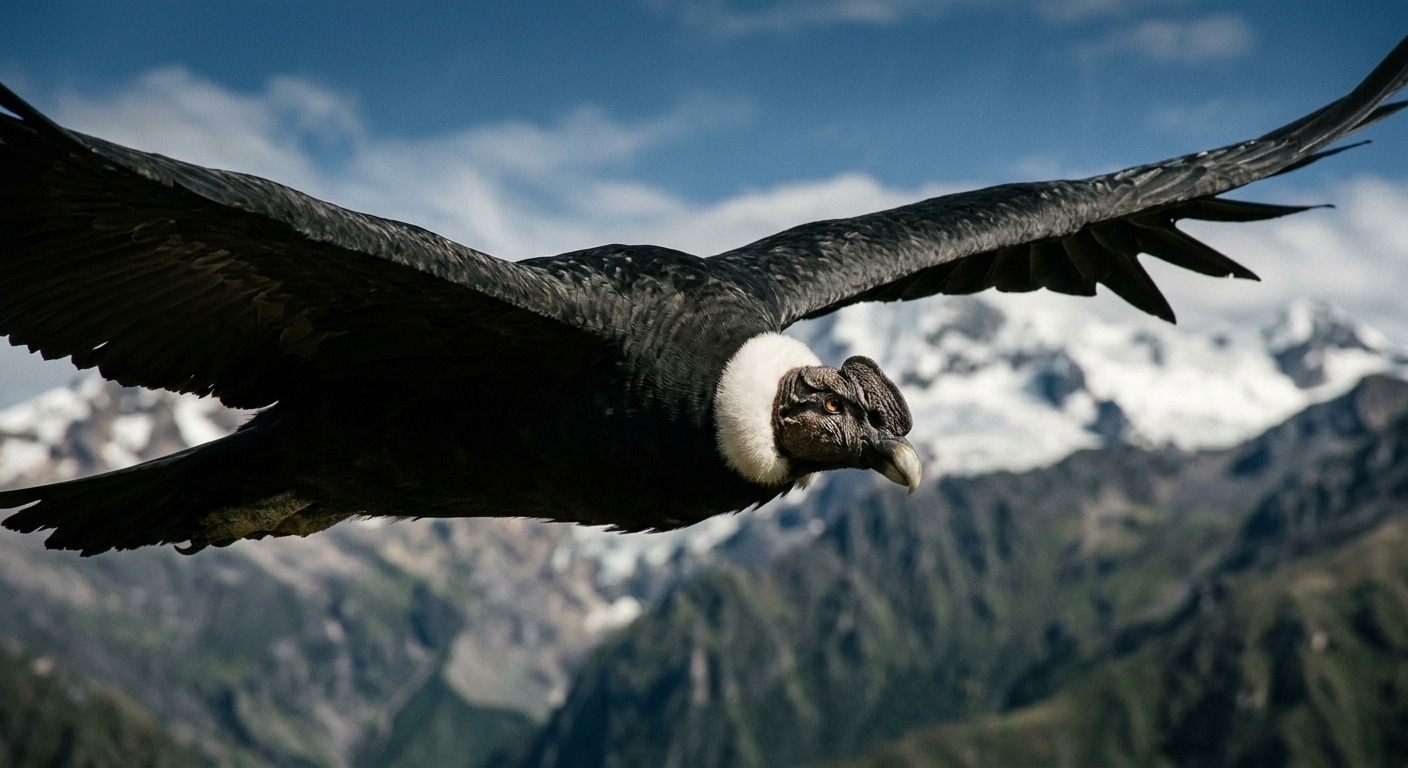
\includegraphics[width=\textwidth,height=1.30cm,keepaspectratio]{../images/TU_IMAGEN_CONDOR.jpg}\\[0.01cm]
			{\small\color{textgray}\itshape\begin{extraer}{condor_sub}Pneuma \corazonrojo: Intuición, espíritu y sentimiento divino \end{extraer}}
		\end{tcolorbox}
	\end{minipage}%
	\hfill
	\begin{minipage}[c]{0.55\textwidth}
		\begin{tcolorbox}[titleBoxStyle, width=\textwidth]
			\centering
			{\Large\color{deepblue}\bfseries\begin{extraer}{main_title}
					El Despertar \cruz
			\end{extraer}}\\[0.01cm]
			\tikz[baseline=-0.5ex]{\draw[golddark, line width=0.7pt] (-2.2,0) -- (2.2,0); \fill[golddark] (0,0) circle (1.5pt);}\\[0.01cm]
			{\small\bfseries\color{golddark}\begin{extraer}{main_sub} Dios es UNO \corazonrojo y Yaldabaoth es EGO \cerebro
			\end{extraer}}
			
			\vspace{0.12cm}
			
			{\fontsize{7.2pt}{8.2pt}\selectfont 
				\begin{extraer}{header_desc}
					
					El vuelo conjunto del Cóndor y del Águila simboliza la unión definitiva entre la ciencia y la espiritualidad, ofreciendo una explicación al denominado arrebatamiento de la Iglesia. El no-tiempo es una propiedad emergente de la pneuma, mientras que el espacio-tiempo es una propiedad emergente de la psyche. Dado que el ego humano posee masa, despojarnos de él equivale a trascender la densidad física para retornar a la luz del Padre Inefable: El Uno
					
					
				\end{extraer}
			}
		\end{tcolorbox}
	\end{minipage}%
	\hfill
	\begin{minipage}[c]{0.215\textwidth}
		\begin{tcolorbox}[sideStyle, width=\textwidth]
			\centering
			{\small\color{deepblue}\bfseries\begin{extraer}{eagle_title}Águila del Norte\end{extraer}}\\[0.01cm]
			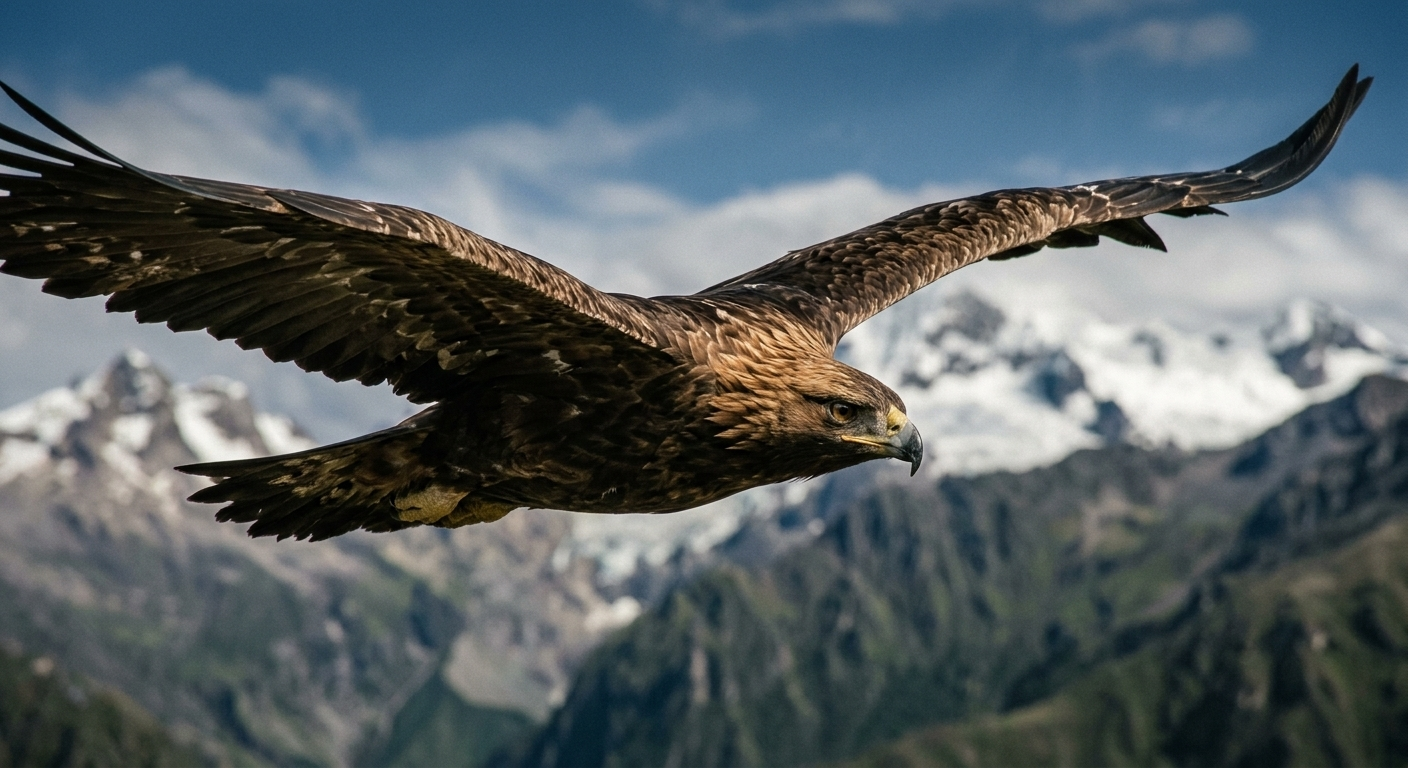
\includegraphics[width=\textwidth,height=1.30cm,keepaspectratio]{../images/TU_IMAGEN_AGUILA.jpg}\\[0.01cm]
			{\small\color{textgray}\itshape\begin{extraer}{eagle_sub}Psyche \cerebro: Ciencia, tecnología y pensamiento material\end{extraer}}
		\end{tcolorbox}
	\end{minipage}
	
	\vspace{0.04cm}
	
	% =========================================================
	% 2. BLOQUE INTRO: CONCIENCIA Y GRAVEDAD CUÁNTICA
	% =========================================================
	\noindent
	\begin{tcolorbox}[introStyle, width=\textwidth]
		\begin{justify}{\fontsize{7.5pt}{8.6pt}\selectfont
				\setstretch{0.88}
				\centering{\bfseries\color{deepblue}\begin{extraer}{left_title}CONCIENCIA DUAL y  GRAVEDAD CUÁNTICA\end{extraer}}\\[0.08cm]
				\begin{extraer}{left_body}
					La Conciencia Primera tiene la misión fundamental de revelarte una verdad oculta: albergas una naturaleza dual y cuántica. La solución a uno de los grandes pilares de la física moderna —la gravedad cuántica— halla su clave en textos redactados hace casi dos milenios: los evangelios gnósticos. En este plano, la conciencia se manifiesta a través de los estados $\vert \text{UNO} \rangle$ y $\vert \text{EGO} \rangle$, lo que revela que poseemos un auténtico libre albedrío de percepción, formalizado matemáticamente mediante el producto interno $\langle \text{UNO} \mid \text{EGO} \rangle$. 
				\end{extraer}
		}\end{justify}
	\end{tcolorbox}
	
	\vspace{0.04cm}
	
	% =========================================================
	% 2b. CITA DE SAGAN (SEPARADA)
	% =========================================================
	\noindent
	\begin{tcolorbox}[saganStyle, width=\textwidth]
		\begin{justify}{\fontsize{7.0pt}{8.2pt}\selectfont\color{textgray}\itshape
				\begin{extraer}{sagan_quote}\enquote{La idea de que Dios es un hombre blanco, más grande de lo normal, con una barba flameante, sentado en el cielo y contando la caída de cada gorrión, es ridícula. Pero si por Dios uno entiende el conjunto de leyes físicas que gobiernan el universo, entonces claramente existe tal Dios. Sin embargo, este Dios es emocionalmente insatisfactorio... no tiene mucho sentido rezarle a la ley de la gravedad}
				\end{extraer}
				\hfill{\small\upshape\color{golddark}\bfseries — Carl Sagan}
		}\end{justify}
	\end{tcolorbox}
	
	\vspace{0.04cm}
	
	% =========================================================
	% 3. TRES COLUMNAS: UNIVERSO DE LUZ | IMAGEN | UNIVERSO MATERIAL
	% =========================================================
	\noindent
	\begin{minipage}[T]{0.25\textwidth}
		\begin{tcolorbox}[contentStyle, width=\textwidth]
			\centering
			{\large\color{deepblue}\bfseries\begin{extraer}{universe_light_title} Pléroma de Luz\end{extraer}}\\[0.05cm]
			{\footnotesize\color{golddark}\bfseries\begin{extraer}{universe_light_sub}UNO \corazonrojo NoTiempo \cruz\end{extraer}}\\[0.01cm]
			\begin{justify}{\fontsize{7.6pt}{8.5pt}\selectfont\color{textgray}
					\begin{extraer}{universe_light_text}
						\textbf{El Padre y yo, uno somos}: Recordar quién eres —la revelación de que el Padre es el universo y de que la muerte no existe— nos libera de la ignorancia. En el hemisferio derecho reside el plano intemporal y divino, la dimensión de alta frecuencia $\vert 999\rangle$. Allí se encuentra la tierra de la unión y la libertad \textit{\textbf{(La Patria Grande)}}.
					\end{extraer}
			}\end{justify}
		\end{tcolorbox}
	\end{minipage}%
	\hfill
	\begin{minipage}[T]{0.50\textwidth}
		\begin{tcolorbox}[centralStyle, width=\textwidth]
			\centering
			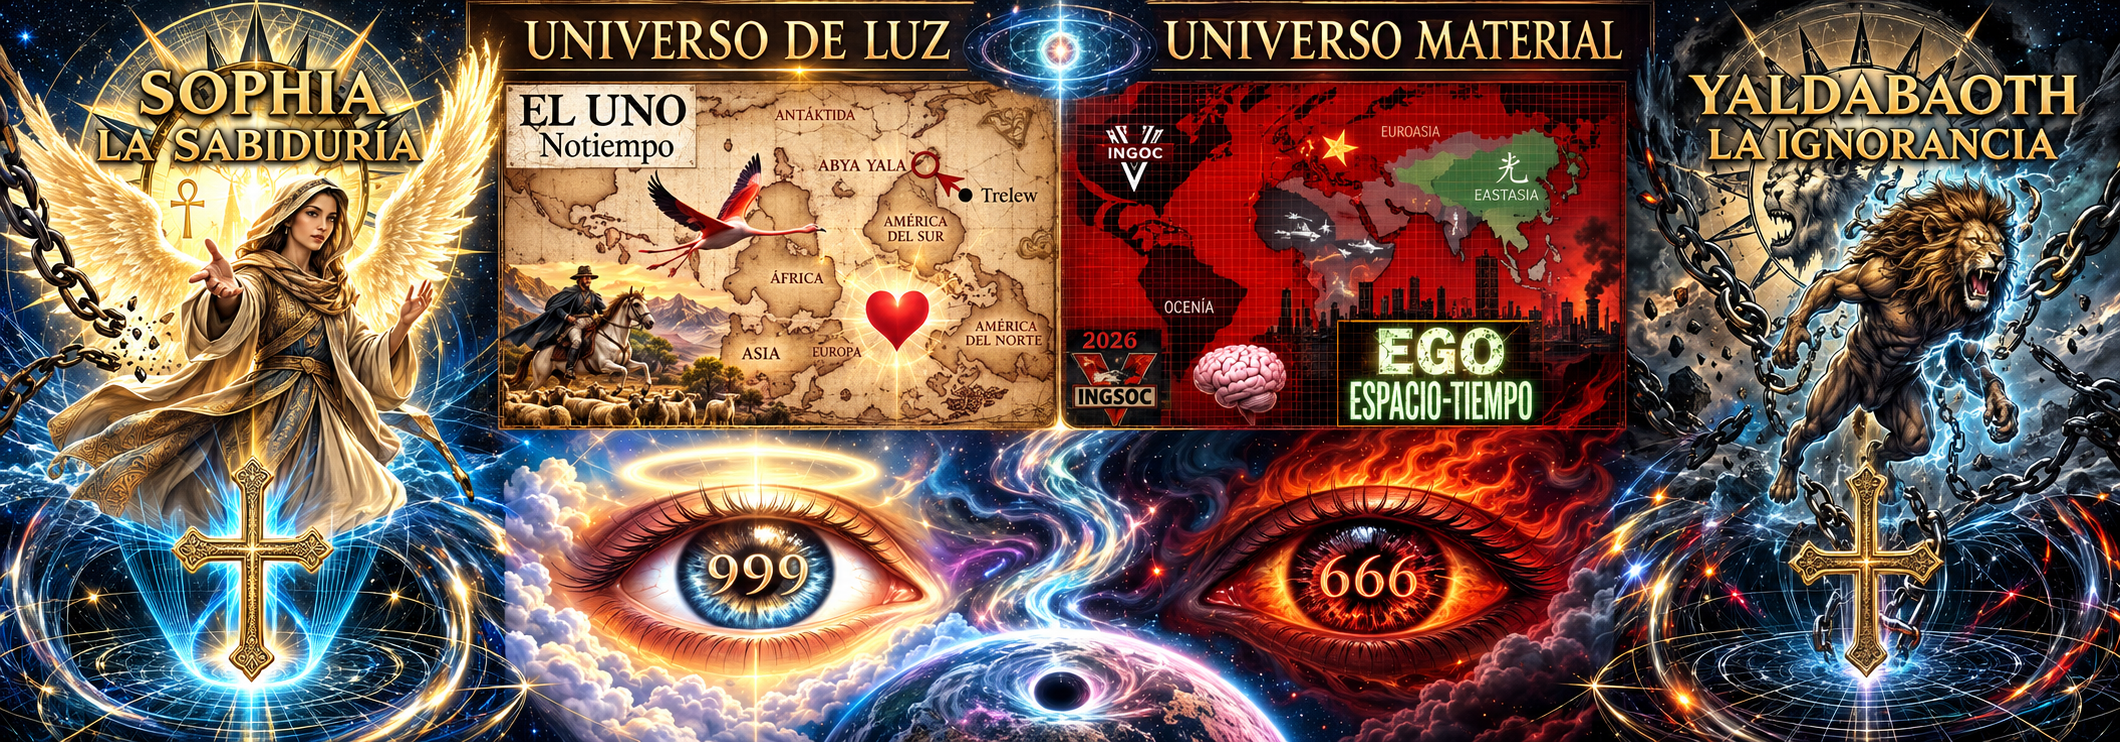
\includegraphics[width=\textwidth,height=4.20cm,keepaspectratio]{../images/sophiavsdemiurgo.png}\\[0.01cm]
			{\scriptsize\color{golddark}\bfseries \begin{extraer}{center_text}
					Sofía, la sabiduría divina, yace atrapada en el caos del mundo material, gobernado por un demiurgo ignorante y cegado por su propio ego.
			\end{extraer}}
		\end{tcolorbox}
	\end{minipage}%
	\hfill
	\begin{minipage}[T]{0.25\textwidth}
		\begin{tcolorbox}[contentStyle, width=\textwidth]
			\centering
			{\large\color{deepblue}\bfseries\begin{extraer}{universe_mat_title} Prisión Material\end{extraer}}\\[0.05cm]
			{\footnotesize\color{golddark}\bfseries\begin{extraer}{universe_mat_sub}EGO \cerebro espaciotiempo \cruzinvertida\end{extraer}}\\[0.01cm]
			\begin{justify}{\fontsize{7.6pt}{8.5pt}\selectfont\color{textgray}
					\begin{extraer}{universe_mat_text}
						El cuerpo humano está compuesto de carbono-12 ($6p^+$, $6e^-$, $6n^0$). En el hemisferio izquierdo radica el plano temporal y material, la dimensión de baja frecuencia $\vert 666\rangle$. La fuerza gravitacional del ego nos arrastran hacia un lugar donde: \enquote{la guerra es la paz, la libertad es la esclavitud y la ignorancia es la fuerza} (1984).
					\end{extraer}
			}\end{justify}
		\end{tcolorbox}
	\end{minipage}
	
	\vspace{0.04cm}
	
	% =========================================================
	% 5. CITA FINAL Y PIE DE PÁGINA
	% =========================================================
	\begin{tcolorbox}[finalQuoteStyle, width=\textwidth]
		{\fontsize{9.2pt}{11.0pt}\selectfont\color{textgray}\itshape
			\enquote{\begin{extraer}{final_quote}Cuando el Águila del Norte y el Cóndor del Sur vuelen juntos en el mismo cielo, la Madre Tierra despertará y la humanidad entera sanará.\end{extraer}}}
	\end{tcolorbox}
	
	\vspace{0.08cm}
	
	\begin{center}
		\vspace{-0.15em}
		\hrule height 0.45pt
		\vspace{0.4em}
		\noindent{\small\textbf{\begin{extraer}{video_title}Documental \enquote{De la Prisión material al Pléroma de luz} \end{extraer}: } \url{https://www.condoryaguila.org}}
	\end{center}
	
\end{document}